% Chapter 2 -- Financial Data and How to Use It Well
% Requires: amsmath, amssymb, booktabs, array, tabularx, longtable, graphicx, tcolorbox (breakable, skins), hyperref or url.
% Defines the callout box only if the preamble has not.
\providecolor{fenavy}{HTML}{1B2A6B}
\providecolor{feshade}{HTML}{F3F5FA}
\makeatletter
\@ifundefined{callout}{%
  \newtcolorbox{callout}{breakable, enhanced,
    colback=white, colframe=gray!70, boxrule=0.5pt, arc=1mm,
    borderline west={2.5pt}{0pt}{gray!70},
    left=8pt, right=8pt, top=4pt, bottom=4pt}%
}{}
\makeatother

\chapter{Financial Data and How to Use It Well}
\label{ch:02}

Chapter~\ref{ch:01} showed what a track record must do to reveal real skill. This chapter turns to what comes first: the data the record is built on. A backtest can test a single idea with honest statistics and still give the wrong answer because of how its dataset was built. The good news is that each problem is well understood, and each has a fix.

The problems are rarely dramatic. Each looks like a technical detail, and each can add a percentage point or more a year to a strategy's measured return:

\begin{itemize}
  \item a price series that is not adjusted for stock splits and dividends, so ordinary corporate events look like gains or losses;
  \item a portfolio that gives a \$20 million company the same weight as a \$2 trillion one, so the result is driven by stocks almost no one can trade in size;
  \item a database that keeps only the companies that still exist, so the failures, and the losses they caused, are missing;
  \item an accounting number used months before it was published, so the strategy trades on information no investor had at the time;
  \item an average return quoted in a way that overstates what an investor actually earned.
\end{itemize}

The claim on trial in this chapter is the one every reader working with free data needs to be true: \textbf{free, public data can support a reliable backtest.} Every lab in this book relies on it, so we test it first, and the answer comes with a checklist that tells you exactly how to make it true.


By the end of the chapter you will be able to:

\begin{itemize}
  \item explain how stock splits and dividends change quoted prices, and why research uses adjusted prices;
  \item compute market capitalization and distinguish value-weighted, equal-weighted and price-weighted portfolios;
  \item describe the main research datasets and their free counterparts, and explain delisting returns and point-in-time data;
  \item choose the right return measure for each task (simple or log, price or total, raw or excess), and explain why arithmetic and geometric averages differ;
  \item recognize survivorship bias, look-ahead bias, micro-cap effects and data snooping, and estimate how much each can distort a result;
  \item apply a data checklist before trusting any backtest.
\end{itemize}

In the lab you will measure four of these problems with nearly a century of real market data and one controlled simulation, see how much each can inflate a strategy's apparent performance, and see how much each fix recovers.

\section{Foundations: where financial data comes from}
\label{sec:02-foundations}

\textbf{Prices, corporate actions and adjusted prices.} A stock's quoted price changes for reasons that are not gains or losses to shareholders. These events are called \textbf{corporate actions}. Two matter most.

\begin{itemize}
  \item \textbf{Stock split.} In a two-for-one split, each share becomes two and the price halves. A shareholder who owned one share at \$100 now owns two shares at \$50: still \$100 in total. A chart of the raw price would show a 50\% ``crash'' that never cost anyone a cent.
  \item \textbf{Dividend.} A dividend pays cash to shareholders. The share price typically falls by roughly the dividend on the \textbf{ex-dividend date}, the first day on which a buyer of the stock no longer receives the payment. If a \$100 stock pays a \$2 dividend and opens at \$98, the price return is $-2$\%, but the shareholder's total return is zero: \$98 in stock plus \$2 in cash.
\end{itemize}

Databases therefore publish \textbf{adjusted prices}, which rescale past prices so that the change in the adjusted price equals the shareholder's return. After the split above, for example, every earlier price is divided by two. Total-return series also adjust for dividends. Data vendors differ in how they adjust, which is one reason two sources can disagree about the same stock's history.

\textbf{Market capitalization and index weights.} A company's \textbf{market capitalization} (or market value) is its share price times the number of shares outstanding: one billion shares at \$50 is a \$50 billion company. How a portfolio uses this number decides which stocks drive its results.

\begin{itemize}
  \item A \textbf{value-weighted} (capitalization-weighted) portfolio holds each stock in proportion to its market capitalization. If company A is worth \$900 billion and company B is worth \$100 billion, together they are worth \$1 trillion, so A receives 90\% of the money invested and B receives 10\%.
  \item An \textbf{equal-weighted} portfolio gives each stock the same share of the money, whatever its size. With the same two companies, A and B each receive 50\%. Company B is only 10\% of the market's value but gets half the portfolio, so equal weighting gives small companies far more influence than their size in the economy.
  \item A \textbf{price-weighted} index, such as the Dow Jones Industrial Average, weights by share price alone. A \$500 stock counts ten times as much as a \$50 stock, whatever the size of the two companies. This is a historical convention with no economic rationale.
\end{itemize}

A value-weighted portfolio needs little rebalancing, because its weights move with prices automatically; it trades mainly when stocks enter or leave the portfolio or companies issue or buy back shares. An equal-weighted portfolio must be rebalanced regularly as prices drift apart, selling part of the stocks that have risen and buying more of those that have fallen to restore equal weights.


\textbf{The main research databases.} Most empirical finance rests on a handful of sources.

\begingroup
\small
\setlength{\LTpre}{6pt}\setlength{\LTpost}{6pt}
\begin{longtable}{@{}>{\raggedright\arraybackslash}p{0.2\linewidth}>{\raggedright\arraybackslash}p{0.42\linewidth}>{\raggedright\arraybackslash}p{0.22\linewidth}@{}}
\toprule
Source & What it holds & Access \\
\midrule
\endfirsthead
\multicolumn{3}{@{}l}{\emph{(continued)}}\\
\toprule
Source & What it holds & Access \\
\midrule
\endhead
\midrule
\multicolumn{3}{r@{}}{\emph{continued on next page}}\\
\endfoot
\bottomrule
\endlastfoot
CRSP (Center for Research in Security Prices) & Daily and monthly returns, prices, shares and delisting information for U.S. stocks since 1926, including companies that no longer exist & Subscription, usually through WRDS \\
Compustat & Company accounting data: balance sheets, income statements, cash flows & Subscription \\
Kenneth R. French Data Library & Factor returns and sorted portfolio returns built from CRSP and Compustat & Free \\
FRED (Federal Reserve Bank of St.\ Louis) & Interest rates, inflation, macroeconomic series; ALFRED holds earlier vintages & Free \\
Exchange and vendor feeds (Yahoo Finance and others) & Recent prices and adjusted prices for currently listed securities & Free or commercial; coverage and adjustment methods vary \\
\end{longtable}
\endgroup

WRDS (Wharton Research Data Services) is the platform through which most universities access CRSP and Compustat. A \textbf{factor} is the return on a portfolio built to capture one source of return, such as small minus large companies. A \textbf{vintage} is a dataset as it stood on a particular date, before later revisions. This book's labs use only free sources. Where a test needs data that only subscription databases hold, such as the returns of companies that delisted, the labs use simulations and say so.

\textbf{Delisting.} A company is \textbf{delisted} when its stock stops trading on an exchange. Companies leave through mergers, going private, moving exchanges or failure. The \textbf{delisting return} is the return from the last trading price to whatever shareholders finally receive. For a failing company it can be large and negative: shareholders may get a few cents a share, or nothing. A database that simply drops delisted companies, or omits their final return, overstates historical returns.

\textbf{Dates and timing.} Accounting data refers to a \textbf{fiscal year}, the company's twelve-month reporting period, which may not end in December. The figures are published weeks or months after the period they describe: a company whose fiscal year ends on 31 December may not publish its annual report until February or March. A study that uses accounting figures as of their reference date rather than their publication date gives itself information no investor had. \textbf{Point-in-time} data records what was known on each date, including the original values of numbers that were later revised.

\section{Measuring returns: choosing the right measure}
\label{sec:02-returns}

Every claim in this book is ultimately a statement about returns, so the way a
return is measured decides what the claim says. The same investment can show
quite different numbers depending on whether dividends are included, whether
the risk-free rate is subtracted and how returns are averaged. Choose the wrong
measure and a strategy can appear to beat the market by several percentage
points a year without earning anything extra.

Section~\ref{sec:01-foundations} defined the simple return
(Equation~\eqref{eq:01-return}), the log return, total and price returns, and
excess returns. This section shows which measure to use for each task. Four
rules cover most cases.

\textbf{Use simple returns across assets and log returns across time.}
Section~\ref{sec:01-foundations} showed that log returns add over time while
simple returns compound. The two measures also add up in different directions.

\begin{itemize}
  \item \textbf{Simple returns add across assets.} A portfolio's simple return is the weighted average of its holdings' simple returns. If half the money earns 10\% and half earns 2\%, the portfolio earns 6\%.
  \item \textbf{Log returns add across time.} A multi-period log return is the sum of the period log returns. Log returns of 5\% and 3\% make 8\% over the two periods.
\end{itemize}

You should therefore use simple returns to build portfolios and log returns for
compounding and for some statistical models. Never mix the two in one
calculation.

\textbf{Compare total return with total return.} A total return includes
dividends and a price return does not (Section~\ref{sec:01-foundations}). Over
long periods the difference is large: dividends have supplied a substantial
share of U.S. stock market returns over the past century. Yet many free
sources, including most stock charts, show price indexes. If you compare a
strategy's total return with an index's price return, the strategy will look
better than it is: it appears to beat the index by the dividend yield, the
annual dividend divided by the price, even when it has no real advantage.
Before comparing any two returns, check that both include dividends.

\textbf{Judge a strategy by its excess return.} Measure performance as the
return above the risk-free rate (Section~\ref{sec:01-foundations}), not as the
raw return. A strategy that earned 5\% when bills paid 5\% added nothing for
the risk it took. The Sharpe ratio and the regressions in later chapters all
use excess returns, so you should compute them from the start.

\textbf{Quote the geometric average when reporting what an investor earned.}
There are two ways to average a series of returns, and they answer different
questions.

\begin{itemize}
  \item The \textbf{arithmetic average}, $A$, is the simple mean of the period returns. It estimates the expected return in any one period.
  \item The \textbf{geometric average}, $G$, is the constant rate that would have produced the same ending wealth. It describes what a buy-and-hold investor actually earned:
  \begin{equation}
    G = \left(\prod_{t=1}^{T} (1 + R_t)\right)^{1/T} - 1
    \label{eq:02-geometric}
  \end{equation}
\end{itemize}

A simple example shows why the choice matters. Suppose an investment gains 50\%
one year and loses 50\% the next. The arithmetic average is $(50 - 50)/2 = 0$\%,
which sounds like breaking even. But \$100 grows to \$150 and then falls to
\$75: the investor lost a quarter of the money. The geometric average is
$\sqrt{1.5 \times 0.5} - 1 \approx -13.4$\% a year, which matches what happened.

The geometric average is always lower than the arithmetic one when returns
vary, and the gap grows with volatility. This gap is often called
\textbf{volatility drag}. You can estimate it with a useful approximation:
\begin{equation}
  G \approx A - \frac{\sigma^2}{2}
  \label{eq:02-drag}
\end{equation}
where $\sigma$ is the volatility. For a stock index with 20\% annual volatility,
the gap is about $0.20^2/2 = 0.02$, or 2 percentage points a year; for a
portfolio of small, volatile stocks with 35\% volatility, it is about 6
(Figure~\ref{fig:02-drag}).

\begin{figure}[htbp]
\centering
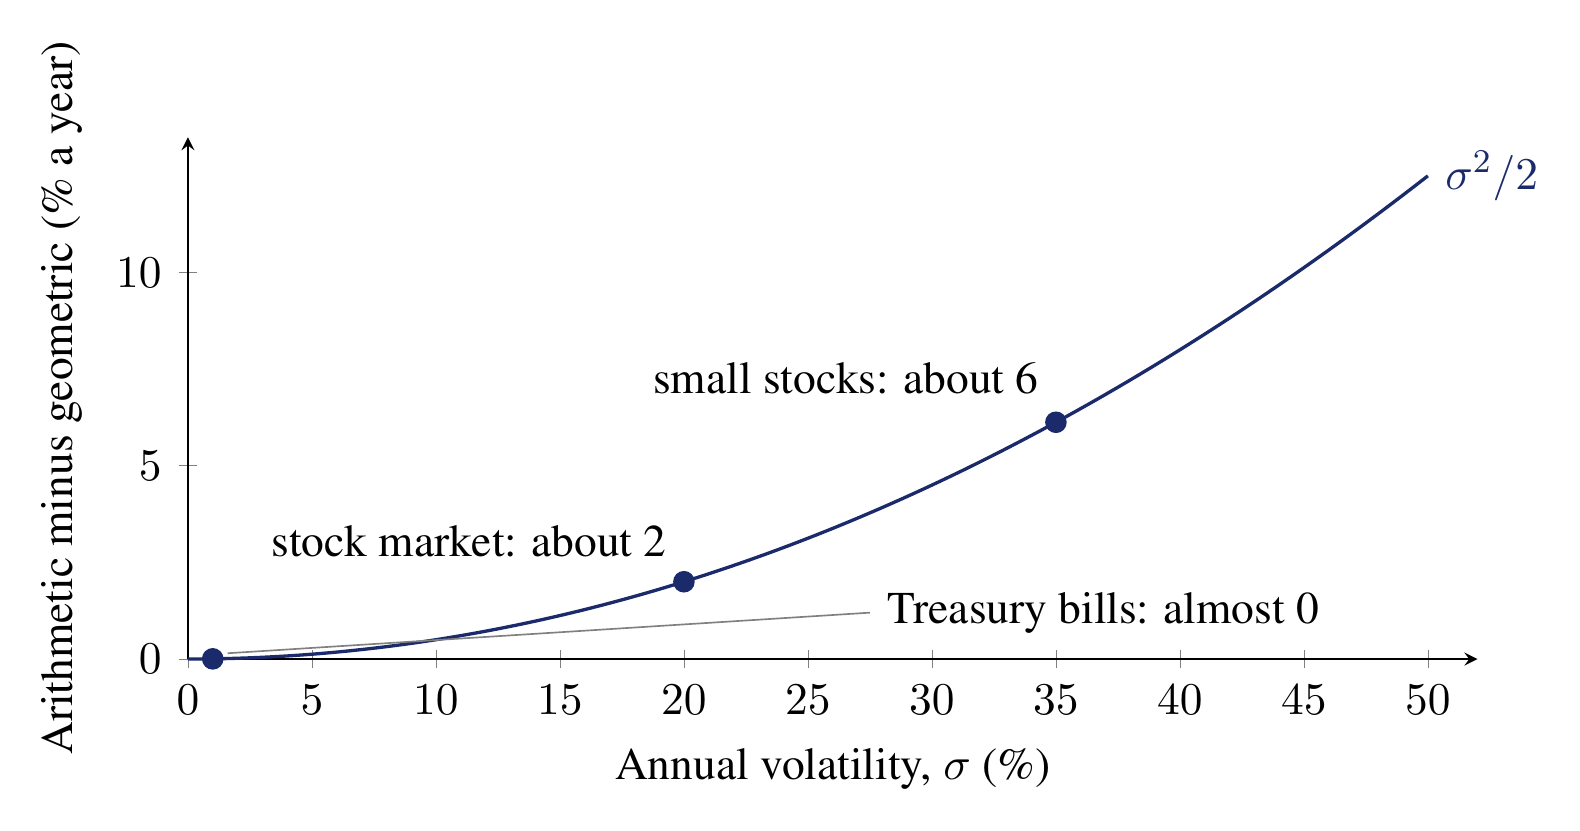
\includegraphics[width=0.85\linewidth]{images/fig02-1-volatility-drag.png}
\caption{Volatility drag: the gap between the arithmetic and geometric average returns, from Equation~\eqref{eq:02-drag}. The gap is negligible for Treasury bills, about 2 percentage points a year for the stock market and about 6 for small stocks, and it rises with the square of volatility.}
\label{fig:02-drag}
\end{figure}

Use the arithmetic average when you need the expected return for a single
period, as in the Sharpe ratio or a forecast. Use the geometric average when you
report how much an investment grew. If you quote the arithmetic average as the
growth rate, you will overstate the investor's experience, and the overstatement
is largest for exactly the volatile strategies that tend to look most
attractive. When a source reports an average return, check which kind it is.
Lab 2 measures the gap on real portfolios.

\section{Research datasets and their free alternatives}
\label{sec:02-datasets}

A result can be no more reliable than the data behind it. Each dataset covers
different companies, periods and events, and each handles corrections,
dividends and failed companies in its own way. If you do not know what your
dataset contains and what it leaves out, you cannot tell whether a result
reflects the market or the database.

Most published research on U.S. stocks rests on the two commercial databases introduced in Section~\ref{sec:02-foundations}, CRSP and Compustat. Two of their features matter most for this chapter, because free sources usually lack them: delisting returns and point-in-time data.


\begin{itemize}
  \item \textbf{CRSP} includes companies that later disappeared, along with the return in the month they delisted.
  \item \textbf{Compustat}'s point-in-time version records what was known on each date, rather than the figures as later revised.
\end{itemize}

Many universities subscribe; many readers will not have access. This book's labs use free sources that are built from, or comparable to, these databases:

\begin{center}
\small
\begin{tabularx}{0.9\linewidth}{@{}>{\raggedright\arraybackslash}p{0.22\linewidth}>{\raggedright\arraybackslash}X>{\raggedright\arraybackslash}p{0.26\linewidth}@{}}
\toprule
Free source & What it offers & Main limitation \\
\midrule
Kenneth R. French Data Library & Factor returns and portfolios sorted on size, value, momentum and more, built from CRSP and Compustat, since 1926 & Portfolio-level only; no individual stocks \\
FRED (Federal Reserve Bank of St.\ Louis) & Interest rates and economic series; its ALFRED archive keeps past vintages of revised data & Economic series, not stock-level data \\
Open Source Asset Pricing (Chen and Zimmermann) & Portfolio returns for over 200 published predictors & Full firm-level signals require WRDS \\
Jensen--Kelly--Pedersen global factors & 153 factors across 93 countries & Factor-level only \\
Yahoo Finance and similar & Daily prices for current stocks, ETFs and indexes & Mostly survivors only; adjustments not always documented; unofficial access methods can break \\
\bottomrule
\end{tabularx}
\end{center}

A \textbf{predictor} (or signal) is a variable, such as a valuation ratio or past return, that a study uses to forecast returns. The last row of the table deserves emphasis. Free stock-price sites are convenient, but they mostly cover companies that exist today. A backtest that pulls today's stocks from such a source and runs them through the past has survivorship bias built in, the problem Section~\ref{sec:02-survivorship} describes.

\section{Survivorship bias: the missing failures}
\label{sec:02-survivorship}

Companies that fail, merge or are delisted disappear from many datasets, and
their final losses disappear with them. A backtest run only on companies that
still exist never suffers those losses, so it overstates returns, often by
several percentage points a year. This is one of the most common errors in
practice, because most free price sources list only today's stocks.

\textbf{Survivorship bias} arises when a sample includes only the companies, funds or strategies that are still around at the end of the period. The ones that failed, were acquired or were shut down disappear from the data, and with them their losses. It is like judging how safe a sport is by interviewing only the players who are still playing.

The bias works through three channels:

\begin{enumerate}
  \item \textbf{Survivors-only samples.} Testing a strategy on today's index members, or on funds that exist today, removes every company or fund that failed along the way. The survivors are, by definition, the ones that did well enough to last.
  \item \textbf{Missing delisting returns.} When a stock leaves the exchange because it is failing, its final return is often large and negative, and often missing from the database. Shumway (1997) showed that CRSP frequently lacked returns for performance-related delistings and estimated that the missing returns averaged about $-30$\% for NYSE and AMEX stocks; Shumway and Warther (1999) found larger losses for Nasdaq stocks. A backtest that silently drops these months overstates returns, most of all for small and distressed stocks.
  \item \textbf{Backfill.} Databases sometimes add a company or fund with its history filled in after it has already succeeded. This \textbf{backfill} brings in past returns only for those that did well. Kothari, Shanken and Sloan (1995) argued that this kind of selection in Compustat inflated the measured returns of high book-to-market stocks, companies whose accounting value is large relative to their market value.
\end{enumerate}

For mutual funds the bias is well documented. Elton, Gruber and Blake (1996) estimated that studying only surviving funds overstated average performance by roughly 0.9 percentage points a year, a large number compared with the alphas researchers try to detect. Brown, Goetzmann, Ibbotson and Ross (1992) showed that survivorship can even make fund performance appear to persist from one period to the next when it does not.

\textbf{Why survivorship can create a strategy out of nothing.} The bias is not just a uniform upward shift. It favors the stocks most likely to fail: small, volatile, \textbf{distressed} companies, those at real risk of bankruptcy. Among those, the survivors are the ones that happened to rise. A survivors-only backtest of a strategy that buys volatile or distressed stocks can therefore show a large premium that is entirely produced by the sample. Lab 2 demonstrates this with a simulation in which the true premium is known to be zero.

\textbf{The fix} is a dataset that includes dead companies and their delisting returns, such as CRSP, and portfolio rules that use only firms listed at each date. When delisting returns are missing, researchers substitute estimates (for example $-30$\%) following Shumway.

\section{Look-ahead bias: using only what was known}
\label{sec:02-lookahead}

A backtest is honest only if every decision uses information that was
available at the time. Accounting figures are published weeks or months after
the period they describe, and economic data are often revised later. Using the
final numbers as if they were known in advance gives a strategy an advantage no
investor had, and the result can look excellent for no real reason.

\textbf{Look-ahead bias} arises when a backtest uses information that was not available at the time the decision would have been made. It is easy to introduce and hard to see, because the code runs without error and the results simply look better than they should. Figure~\ref{fig:02-timeline} shows the most common case: accounting data used before it was published.

\begin{figure}[htbp]
\centering
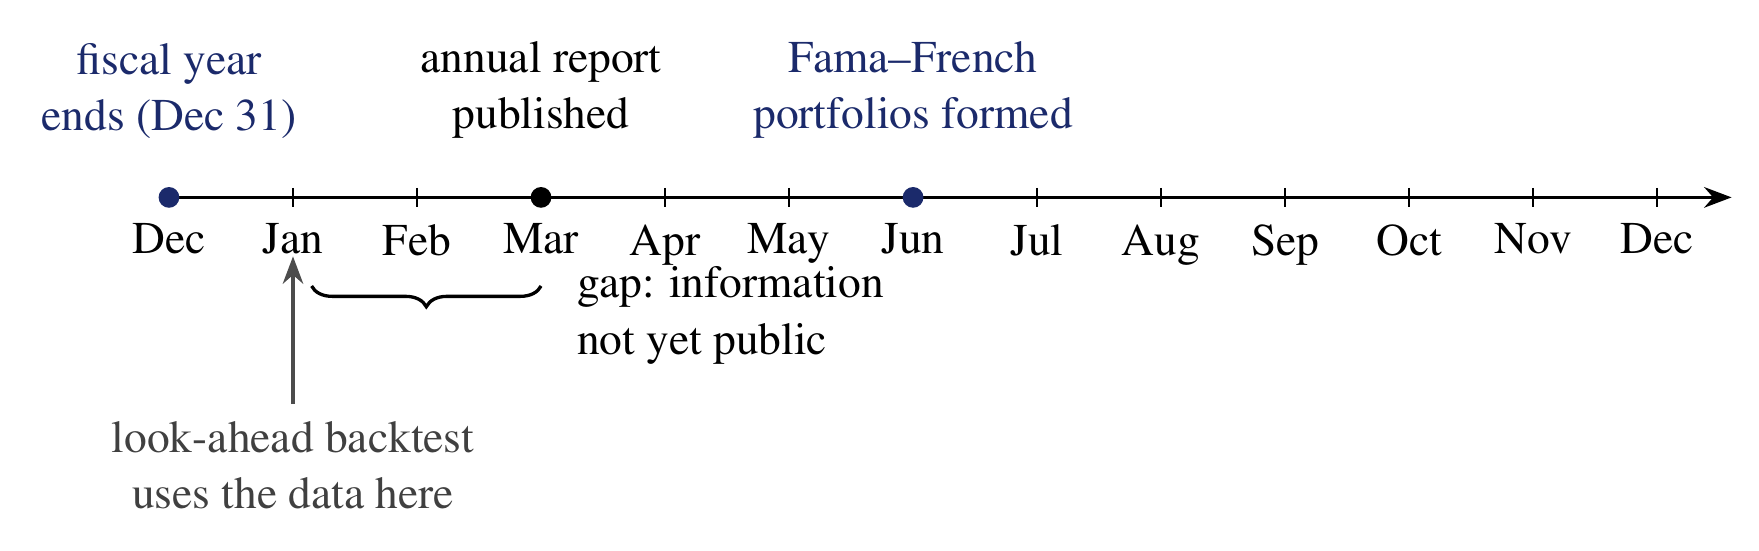
\includegraphics[width=0.9\linewidth]{images/fig02-2-accounting-timeline.png}
\caption{When accounting data becomes usable. A company's fiscal year ends in December, but its annual report appears only months later. A backtest that trades on the figures in January uses information no investor had. Fama and French wait until the following June to be safe.}
\label{fig:02-timeline}
\end{figure}

Common sources, and the standard defense against each:

\begin{center}
\small
\begin{tabularx}{0.9\linewidth}{@{}>{\raggedright\arraybackslash}p{0.16\linewidth}>{\raggedright\arraybackslash}X>{\raggedright\arraybackslash}p{0.32\linewidth}@{}}
\toprule
Source & What goes wrong & Standard defense \\
\midrule
Same-period execution & A signal computed from today's closing price is used to trade at that same close & Trade on the next period's return: lag every signal by at least one period \\
Accounting publication lags & Annual results for a December fiscal year are used in January, though they are published weeks or months later & Lag accounting data; Fama and French (1993) use fiscal-year data only from the following June \\
Revised economic data & GDP or employment figures are used as revised years later, not as first reported & Use real-time vintages, such as FRED's ALFRED archive \\
Index membership & Today's index members are used for the past & Use historical membership lists \\
Full-sample choices & Parameters, thresholds or variable definitions are chosen using the whole sample, then ``tested'' on it & Choose using only data available at each date (walk-forward; Chapter 5) \\
Full-sample scaling & Signals are standardized with means and volatilities computed over the whole sample & Use expanding or rolling estimates \\
\bottomrule
\end{tabularx}
\end{center}

Three terms in the table need a word of explanation. To \textbf{lag} a signal is to use it only from a later period, so that it was known before the trade. A \textbf{walk-forward} test chooses its settings at each date using only data before that date, as an investor in real time would have to. An \textbf{expanding} estimate uses all data up to each date; a \textbf{rolling} one uses a fixed window, such as the past five years.

The last two rows are the subtlest. No future price is used directly, yet the analyst's choices encode knowledge of how the whole period turned out. A trading rule whose window length was picked because it worked best over 1926--2025 carries information from 2025 back into 1926.

\textbf{Point-in-time data} is the general remedy: for each date, use only the values that were knowable then. Lab 2 measures two forms of look-ahead on real data: trading on the same day's close, and choosing a rule's parameter with hindsight.

\section{Micro-caps: results no investor could capture}
\label{sec:02-microcaps}

The smallest companies are costly or impossible to trade in size, yet in an
equal-weighted portfolio they carry the same weight as the largest. A result can
therefore be driven almost entirely by stocks no investor could realistically
buy. Checking how a portfolio is weighted, and whether the result survives
without the smallest stocks, is one of the quickest tests of whether a finding
is usable.

The U.S. stock market is extremely unequal. A few hundred large companies make up most of its value, while thousands of tiny companies make up most of its names. Fama and French (2008) classified stocks below the 20th percentile of NYSE market capitalization as \textbf{micro-caps}, meaning companies smaller than four-fifths of the stocks listed on the New York Stock Exchange. They found that micro-caps were about 60\% of all listed stocks but only about 3\% of total market value (Figure~\ref{fig:02-microcaps}).

\begin{figure}[htbp]
\centering
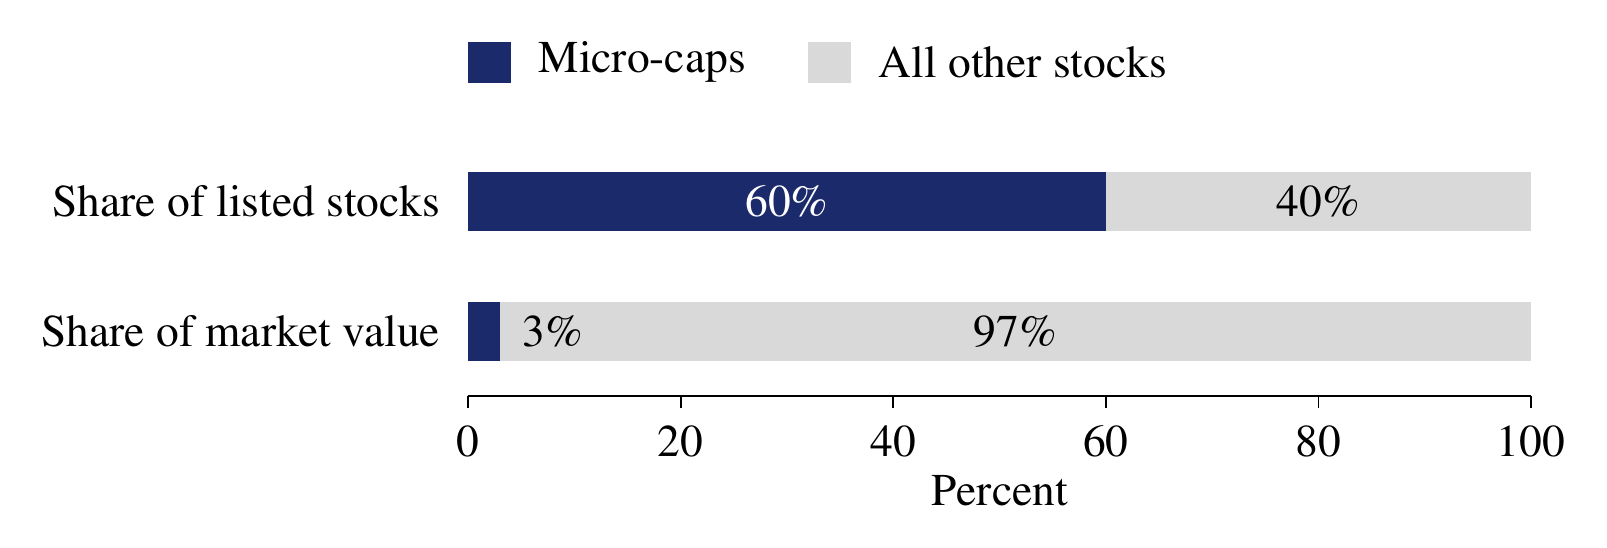
\includegraphics[width=0.8\linewidth]{images/fig02-3-microcaps.png}
\caption{Micro-caps are most of the stocks but almost none of the money. Source: Fama and French (2008).}
\label{fig:02-microcaps}
\end{figure}

This matters because of how portfolios are weighted (Section~\ref{sec:02-foundations}):

\begin{itemize}
  \item \textbf{Equal-weighted} portfolios give every stock the same weight, so micro-caps dominate them by number.
  \item \textbf{Value-weighted} portfolios weight stocks by market capitalization, so they reflect where investors' money actually is.
\end{itemize}

Micro-caps are expensive and difficult to trade. Their \textbf{bid--ask spreads}, the gap between the price at which you can buy and the price at which you can sell, are wide. They have little \textbf{liquidity}: buying or selling even a modest amount moves the price. And they are costly to \textbf{sell short}, that is, to borrow and sell in the hope of buying back more cheaply. They also have the most extreme returns and the most data problems, including the missing delisting returns of Section~\ref{sec:02-survivorship}. A pattern that appears in equal-weighted portfolios but not value-weighted ones may exist only where no large investor can exploit it.

The replication debate in Chapter 10 turns partly on this point. An \textbf{anomaly} is a pattern in returns that standard risk models, such as the CAPM, cannot explain. Hou, Xue and Zhang (2020) found that many anomalies fail when micro-caps are given little weight; their critics argue that this mainly shows anomalies are concentrated among small stocks. Either way, the lesson for this chapter is simple: \textbf{always ask how a portfolio is weighted and whether the result survives without micro-caps.}

\begin{callout}
\textbf{What Failed: the size effect.} Banz (1981) found that small companies had earned higher risk-adjusted returns than large ones, and ``small beats big'' became one of the best-known findings in finance. Later research found the effect much weaker after its publication, heavily concentrated among the very smallest stocks, and in early studies concentrated in January. Size remains a common factor in models of risk, but as a stand-alone source of extra return it has been far less reliable than its early evidence suggested. Lab 2 tests how much of the size premium comes from micro-caps and from the years before 1981.
\end{callout}

\section{Data snooping: when a whole field searches one dataset}
\label{sec:02-snooping}

Chapter 1 described selection within one researcher's search. There is a wider version: an entire field searching the same data. Most U.S. stock research uses CRSP, much of it the same post-1963 period. Thousands of researchers have tested thousands of ideas on it, and the ideas that ``worked'' were published. Each paper may report a single, honest test, yet collectively the field has run an enormous number of trials on one history. A finding can therefore be a false discovery even when its author did nothing wrong, which is why a result must be confirmed on data that played no part in finding it.

Lo and MacKinlay (1990) called this \textbf{data-snooping bias}: when the choice of what to test is influenced by what earlier studies found in the same data, standard significance levels overstate the evidence. The bias cannot be fixed by any single researcher, because no one knows how many ideas were tried and abandoned across the field.

Three defenses work, and later chapters use all of them:

\begin{enumerate}
  \item \textbf{New data.} Test the claim in periods or markets that played no part in its discovery: before the original sample, after publication, or in other countries (Chapters 8--10).
  \item \textbf{Higher hurdles.} Require stronger evidence for claims tested on heavily used data, such as a t-statistic above 3 (Harvey, Liu and Zhu 2016; Chapter 4).
  \item \textbf{Economic reasoning stated in advance.} A claim backed by a mechanism specified before the test is less likely to be a statistical accident than one explained after the fact.
\end{enumerate}

\section{Lab 2: Four ways data can mislead}
\label{sec:02-lab}

\begin{callout}
\textbf{Lab 2 at a glance.} \emph{Claim on trial:} free, public data can support a reliable backtest. \emph{Data:} monthly and daily U.S. market returns and size-sorted portfolios since 1926, from the Kenneth R. French Data Library (downloaded automatically), plus a simulated stock market. \emph{Tools:} Python with pandas, NumPy and matplotlib, plus the fintest module. \emph{Time:} about 90 minutes, including the guided notebook. \emph{Code:} repository folder \texttt{ch02-data-traps/}.
\end{callout}

The lab measures each problem from Sections~\ref{sec:02-returns} to~\ref{sec:02-microcaps} in turn. Three parts use real data. Survivorship uses a simulation, for a reason that is itself part of the lesson: free data sources do not include the companies that disappeared, which is exactly the data needed to measure the bias.

\subsection*{Part A: Arithmetic versus geometric averages}

\textbf{Predict first.} Write down which of four portfolios you expect to show
the largest gap between its arithmetic and geometric average returns, and
roughly how large.

The lab computes both averages for Treasury bills, the stock market, and the
largest and smallest 10\% of stocks, annualizing each in the same way so the
comparison is like for like. It then compares each measured gap with the
volatility-drag approximation from Section~\ref{sec:02-returns}: the geometric
average is roughly the arithmetic average minus half the variance,
$G \approx A - \sigma^2/2$ (Figure 2.4). Expect almost no gap for Treasury
bills, about 2 percentage points a year for the market, and the largest gap,
several points a year, for the smallest stocks. If the measured and approximate
gaps differ, ask why: the approximation assumes returns are close to normal,
and small stocks are not.

\subsection*{Part B: Survivorship bias in a market where the truth is known}

\textbf{Predict first.} Before running this part, write down how much you
expect survivorship bias to add to the market's average return each year.

With real data we never know the true answer, so the lab builds a market where
we do. It simulates about 2,000 listed companies over 30 years, and every
company has the \textbf{same expected return}: no stock or strategy has a real
advantage. A company whose price falls below 20\% of its listing price is
delisted with a final return of $-30$\%, following Shumway (1997). Other
companies are acquired at a premium, and every company that leaves is replaced
by a new listing.

From this one simulated history, the lab builds three datasets:

\begin{center}
\small
\begin{tabularx}{0.9\linewidth}{@{}>{\raggedright\arraybackslash}p{0.26\linewidth}>{\raggedright\arraybackslash}X>{\raggedright\arraybackslash}p{0.28\linewidth}@{}}
\toprule
Dataset & What it contains & Real-world equivalent \\
\midrule
Full data & Every company, including its delisting return & CRSP, used correctly \\
Missing delisting returns & Every company, but without the final delisting month & A database with gaps in delisting returns \\
Survivors only & Only companies still listed at the end & Today's stocks downloaded from a free price site \\
\bottomrule
\end{tabularx}
\end{center}

On each dataset, the lab measures two things: the equal-weighted market return,
and the return of a strategy that each month buys the most volatile fifth of
stocks and sells the least volatile fifth, sorted on past volatility only
(Figure 2.5). The full data give the true answer. Any difference in the other
two datasets comes entirely from how they were built.

With the lab's default settings (2,000 listed companies, 30 years, seed 2026),
5,856 companies are listed over the period, 1,693 are delisted for poor
performance, and 2,000 survive to the end. The results:

\begin{center}
\small
\begin{tabularx}{0.9\linewidth}{@{}>{\raggedright\arraybackslash}X>{\raggedright\arraybackslash}p{0.22\linewidth}>{\raggedright\arraybackslash}p{0.22\linewidth}r@{}}
\toprule
Dataset & Equal-weighted compound return & Volatile minus calm, per year & t-statistic \\
\midrule
Full data & 9.3\% & $-1.2$\% & $-2.2$ \\
Missing delisting returns & 10.7\% & $+2.0$\% & 3.5 \\
Survivors only & 14.0\% & $+12.0$\% & 14.7 \\
\bottomrule
\end{tabularx}
\end{center}

Read the table from top to bottom. In the full data, the volatile-minus-calm
strategy loses about 1\% a year, because volatile companies are delisted more
often. Leaving out only the delisting returns flips the sign: the strategy now
appears to earn 2\% a year. Keeping only the survivors adds almost five
percentage points a year to the market's return and creates a ``volatility
premium'' of 12\% a year, with a t-statistic far beyond any hurdle in this book.
None of it is real. Compare these numbers with your prediction.

\subsection*{Part C: Look-ahead bias}

\textbf{Predict first.} Write down whether you expect a one-day timing error to
change a strategy's Sharpe ratio a little or a lot.

\textbf{C1. Trading on the same day's close.} Test a classic timing rule: hold
stocks when the market closes above its 200-day \textbf{moving average}, the
average closing price over the past 200 trading days, and hold Treasury bills
otherwise. Run it two ways. The correct version decides at yesterday's close and
earns today's return. The look-ahead version decides at today's close but is
still credited with today's return. The difference is a single day, the kind of
error that can hide in one misplaced line of code. Compare the two versions'
returns and Sharpe ratios (Figure 2.6).

\textbf{C2. Choosing the window with hindsight.} Now test moving-average windows
from 20 to 300 days, and choose one in two ways. The hindsight version picks the
window with the best Sharpe ratio over the whole evaluation period. The
walk-forward version picks, each January, the window that had worked best up to
that point, using only past data (Figure 2.7). The gap between the two measures
how much a result is inflated by choosing a rule's settings after seeing the
results.

\subsection*{Part D: Micro-caps, weighting and the size premium}

\textbf{Predict first.} Write down whether you expect the size premium to be
larger in value-weighted or equal-weighted portfolios, and whether it survives
after 1981.

Using size-sorted portfolios, the lab measures the \textbf{size premium}, the
return of the smallest tenth of stocks minus the largest tenth, four ways:
value-weighted and equal-weighted, and with and without the smallest tenth of
stocks. It then splits the sample before and after Banz's 1981 publication
(Figure 2.8). Together these test the What Failed box in
Section~\ref{sec:02-microcaps} directly: if the premium lives mainly in tiny,
hard-to-trade stocks or disappears after it was published, the claim weakens.

\emph{[Draft note: figures and numbers for Parts A, C and D are generated from the Kenneth R. French data at the time of publication; the book prints those results. The Part B simulation is fixed by design and its results can be printed as they stand.]}

\subsection*{Your verdict}

Readers write one sentence per problem, saying how much it changed the result and in which direction, and then judge the claim. The expected verdict is \textbf{survives, with conditions}. Free data can support a reliable backtest when you:

\begin{enumerate}
  \item use total returns and compare them with a total-return benchmark, quoting the geometric average for growth (Part A);
  \item use data that include failed companies, such as the French library's portfolios, which are built from CRSP, rather than a list of today's stocks (Part B);
  \item lag every signal and every accounting figure, and choose a rule's settings with walk-forward tests (Part C);
  \item check that the result survives value weighting and the removal of micro-caps (Part D).
\end{enumerate}

A backtest that skips these steps can look excellent and mean nothing; one that follows them can be trusted as far as its statistics allow. The checklist in the next section turns these conditions into questions you can ask of any backtest, including your own.

\section{What investors can use: a data checklist}
\label{sec:02-checklist}

Before trusting any backtest, your own or someone else's, run through these questions. Each maps to a section of this chapter, and most can be answered in a few minutes.

\begin{itemize}
  \item[$\square$] \textbf{Returns (Section~\ref{sec:02-returns}):} Are returns total returns, including dividends? Are they compared with a total-return benchmark? Is the reported average arithmetic or geometric?
  \item[$\square$] \textbf{Excess returns (Section~\ref{sec:02-returns}):} Is performance measured above the risk-free rate?
  \item[$\square$] \textbf{Survivorship (Section~\ref{sec:02-survivorship}):} Does the dataset include companies or funds that no longer exist? Are delisting returns included?
  \item[$\square$] \textbf{Look-ahead (Section~\ref{sec:02-lookahead}):} Is every signal lagged so it uses only information available before the trade? Are accounting data lagged to their publication dates?
  \item[$\square$] \textbf{Hindsight choices (Section~\ref{sec:02-lookahead}):} Were parameters, thresholds or universes chosen using the whole sample?
  \item[$\square$] \textbf{Weighting (Section~\ref{sec:02-microcaps}):} Is the portfolio value- or equal-weighted? Does the result survive without micro-caps?
  \item[$\square$] \textbf{Shared data (Section~\ref{sec:02-snooping}):} Has the result been tested on data that played no part in its discovery: other periods, other markets, or after publication?
\end{itemize}

\textbf{Questions to ask a fund manager or strategy vendor}

\begin{itemize}
  \item Which database was the backtest built on, and does it include delisted stocks and delisting returns?
  \item How were signals lagged, and when would each piece of data actually have been available?
  \item Is the strategy value- or equal-weighted, and what share of its return comes from the smallest stocks?
  \item Is the reported return arithmetic or compound, and before or after costs?
\end{itemize}

\section*{Exercises}
\addcontentsline{toc}{section}{Exercises}

\subsection*{Conceptual (all readers)}

\begin{enumerate}
  \item A strategy reports an average annual return of 18\% with volatility of 40\%. Estimate its geometric average. Which number should an investor care about, and why?
  \item Explain why a portfolio's simple return is a weighted average of its holdings' simple returns, while a multi-period return is a sum of log returns.
  \item A researcher backtests a strategy on the stocks in today's S\&P 500 index from 2005 to today. List two biases in this design and the direction of each.
  \item A study uses annual accounting data for fiscal years ending in December and forms portfolios in January of the next year. What is the problem, and how do Fama and French avoid it?
  \item Explain why survivorship bias can create a premium for volatile stocks, not just raise all returns equally.
  \item A paper reports a strong anomaly in equal-weighted portfolios that disappears in value-weighted ones. What does this suggest about who could profit from it?
\end{enumerate}

\subsection*{Lab extensions (technical readers)}

\begin{enumerate}
  \setcounter{enumi}{6}
  \item Re-run Part B with a delisting return of $-55$\%, closer to estimates for Nasdaq stocks. How do the three datasets change?
  \item In Part C, try windows of 50 and 300 days. Is the look-ahead gain larger for fast or slow rules? Explain.
  \item In Part C, charge a trading cost of 0.1\% each time the rule switches. Does the correctly traded rule still beat buy-and-hold on a risk-adjusted basis?
  \item In Part D, move the publication split to 1990 and 2000. When does the size premium appear to fade?
  \item \textbf{Challenge:} using a free price source, backtest an equal-weighted portfolio of today's S\&P 500 members over the past 20 years and compare it with the equal-weighted S\&P 500 index. Which problem from this chapter explains the difference?
\end{enumerate}

\section*{References}
\addcontentsline{toc}{section}{References}

\begin{itemize}
  \item Banz, R. W. (1981). The Relationship Between Return and Market Value of Common Stocks. \emph{Journal of Financial Economics} 9(1): 3--18.
  \item Brown, S. J., Goetzmann, W., Ibbotson, R. G. and Ross, S. A. (1992). Survivorship Bias in Performance Studies. \emph{Review of Financial Studies} 5(4): 553--580.
  \item Elton, E. J., Gruber, M. J. and Blake, C. R. (1996). Survivorship Bias and Mutual Fund Performance. \emph{Review of Financial Studies} 9(4): 1097--1120.
  \item Fama, E. F. and French, K. R. (1993). Common Risk Factors in the Returns on Stocks and Bonds. \emph{Journal of Financial Economics} 33(1): 3--56.
  \item Fama, E. F. and French, K. R. (2008). Dissecting Anomalies. \emph{Journal of Finance} 63(4): 1653--1678.
  \item Harvey, C. R., Liu, Y. and Zhu, H. (2016). \ldots and the Cross-Section of Expected Returns. \emph{Review of Financial Studies} 29(1): 5--68.
  \item Hou, K., Xue, C. and Zhang, L. (2020). Replicating Anomalies. \emph{Review of Financial Studies} 33(5): 2019--2133.
  \item Kothari, S. P., Shanken, J. and Sloan, R. G. (1995). Another Look at the Cross-Section of Expected Stock Returns. \emph{Journal of Finance} 50(1): 185--224.
  \item Lo, A. W. and MacKinlay, A. C. (1990). Data-Snooping Biases in Tests of Financial Asset Pricing Models. \emph{Review of Financial Studies} 3(3): 431--467.
  \item Shumway, T. (1997). The Delisting Bias in CRSP Data. \emph{Journal of Finance} 52(1): 327--340.
  \item Shumway, T. and Warther, V. A. (1999). The Delisting Bias in CRSP's Nasdaq Data and Its Implications for the Size Effect. \emph{Journal of Finance} 54(6): 2361--2379.
\end{itemize}

\textbf{Data:} Kenneth R. French Data Library: Fama/French 3 Factors (monthly and daily); Portfolios Formed on Size. \url{https://mba.tuck.dartmouth.edu/pages/faculty/ken.french/data_library.html}
